\documentclass[11pt,a4paper]{article}

\usepackage[utf8]{inputenc}
\usepackage[margin=0.85in]{geometry}
\usepackage{amsmath,amssymb,amsfonts}
\usepackage{graphicx}
\usepackage{xcolor}
\usepackage{subcaption}
\usepackage{float}
\usepackage{hyperref}
\usepackage{booktabs}
\usepackage{microtype}
\usepackage{tabularx}
\usepackage{array}
\usepackage{booktabs}

\hypersetup{
    colorlinks=true,
    linkcolor=blue!70!black,
    citecolor=blue!70!black,
    urlcolor=blue!70!black
}

\title{\textbf{\Large Part 1: Interactive Segmentation via Intelligent Scissors and Marr-Hildreth Edge Detection}}
\author{}
\date{}

\begin{document}

\maketitle

The \textbf{Intelligent Scissors} method formulates interactive segmentation as a shortest-path problem on a weighted graph. Each pixel is a vertex connected to its 8-connected neighbors, and edge costs are based on gradient magnitude, gradient orientation, and Laplacian of Gaussian zero-crossings. Dijkstra's algorithm finds paths that follow object boundaries. This report covers:

\begin{enumerate}
    \item \textbf{Edge Detection:} Implementing Marr-Hildreth filtering and studying $\sigma$ and threshold $t$.
    \item \textbf{Graph and Costs:} Combining zero-crossing, gradient magnitude, and orientation features.
    \item \textbf{Shortest Paths:} Applying Dijkstra's algorithm and comparing four cost configurations.
    \item \textbf{Segmentation:} Connecting manually selected seeds and generating a binary mask.
    \item \textbf{Modifications:} Comparing Canny edges and alternative feature weights.
\end{enumerate}

\begin{figure}[H]
    \centering
    \begin{subfigure}[b]{0.48\textwidth}
        \centering
        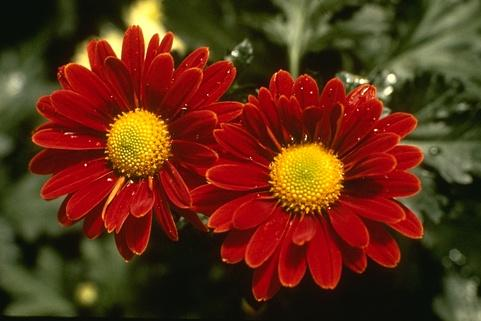
\includegraphics[width=\linewidth]{image1/input.jpg}
        \caption{Original input photograph ($321 \times 481$)}
    \end{subfigure}
    \hfill
    \begin{subfigure}[b]{0.42\textwidth}
        \centering
        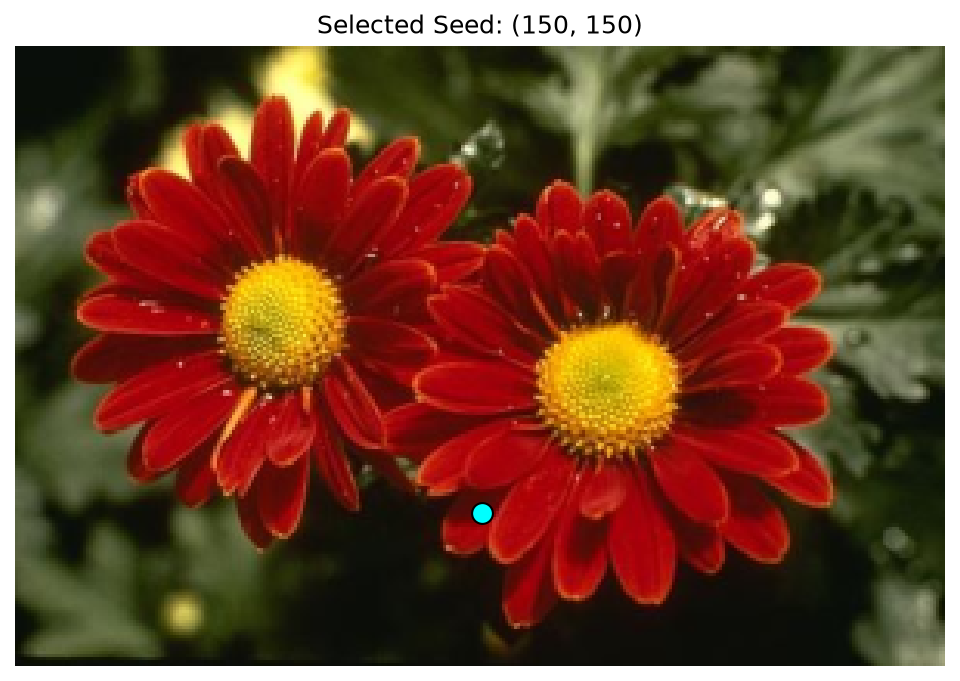
\includegraphics[width=\linewidth]{image1/seed.png}
        \caption{Resized workspace ($200 \times 300$) with test seed}
    \end{subfigure}
    \caption{Input photograph of cosmos flowers and resized image used for segmentation.}
    \label{fig:input}
\end{figure}


\section{Marr-Hildreth Edge Detection}

\subsection{Mathematical Formulation}

The Marr-Hildreth detector identifies edges at zero-crossings of the second derivative of a smoothed image. The image $I(x,y)$ is first smoothed using a 2D Gaussian kernel:

\[
G_\sigma(x,y) = \frac{1}{2\pi\sigma^2}
\exp\left(-\frac{x^2+y^2}{2\sigma^2}\right)
\]

Applying the Laplacian is equivalent to convolving the original image with the \textbf{Laplacian of Gaussian (LoG)} kernel:

\[
\nabla^2(I * G_\sigma) = I * (\nabla^2 G_\sigma)
\]

where

\[
\nabla^2 G_\sigma(x,y) =
\frac{x^2+y^2-2\sigma^2}{2\pi\sigma^6}
\exp\left(-\frac{x^2+y^2}{2\sigma^2}\right)
\]

We compute the LoG response in discrete space using SciPy's Gaussian Laplace function. The parameter $\sigma$ controls the smoothing scale.

\subsection{Zero-Crossing Detection and Slope Thresholding}

A pixel is marked as a zero-crossing when its LoG response has the opposite sign to that of an 8-connected neighbor. We retain the crossing only when the absolute response difference is at least the \textbf{slope threshold} $t$:

\[
\text{crossing}(x,y) = \bigvee_{(dx,dy)\in N_8}
\left[
\text{LoG}(x,y)\text{LoG}(x+dx,y+dy)<0
\;\land\;
|\text{LoG}(x,y)-\text{LoG}(x+dx,y+dy)|\ge t
\right]
\]

Figure below shows the grayscale image, LoG response, and binary zero-crossing map for $\sigma=1.5$ and $t=0.03$.

\begin{figure}[H]
    \centering
    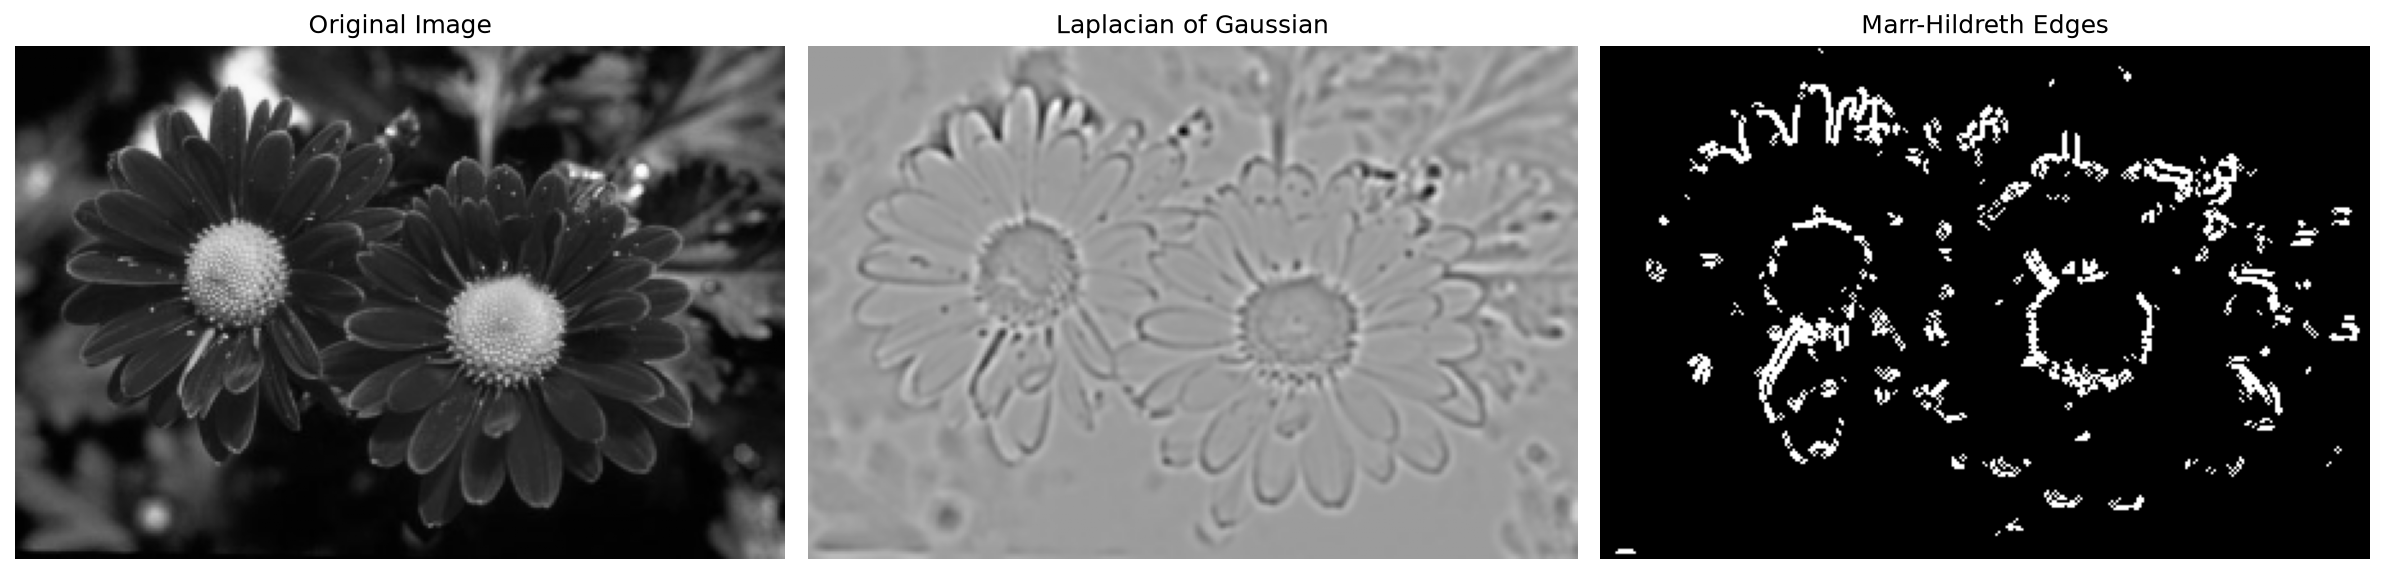
\includegraphics[width=\linewidth]{image1/marr_hildreth.png}
    \caption{Marr-Hildreth edge detection: grayscale input (left), LoG response (center), and binary zero-crossing map (right), using $\sigma=1.5$ and $t=0.03$.}
    \label{fig:marr_hildreth}
\end{figure}

\subsection{Parameter Sensitivity Analysis}

We study the effects of the Gaussian smoothing radius $\sigma$ and slope threshold $t$ by varying each while keeping the other fixed.

\subsubsection{Effect of Gaussian Smoothing Radius ($\sigma$)}

Figure below compares $\sigma \in \{0.5,1.5,2.5\}$ at fixed $t=0.015$:
\begin{itemize}
    \item \textbf{$\sigma=0.5$:} Fine details remain visible, but noise creates many false edges.
    \item \textbf{$\sigma=1.5$:} Noise is reduced while the main flower boundary remains clear.
    \item \textbf{$\sigma=2.5$:} Strong smoothing merges nearby edges and reduces boundary localization.
\end{itemize}

\begin{figure}[H]
    \centering
    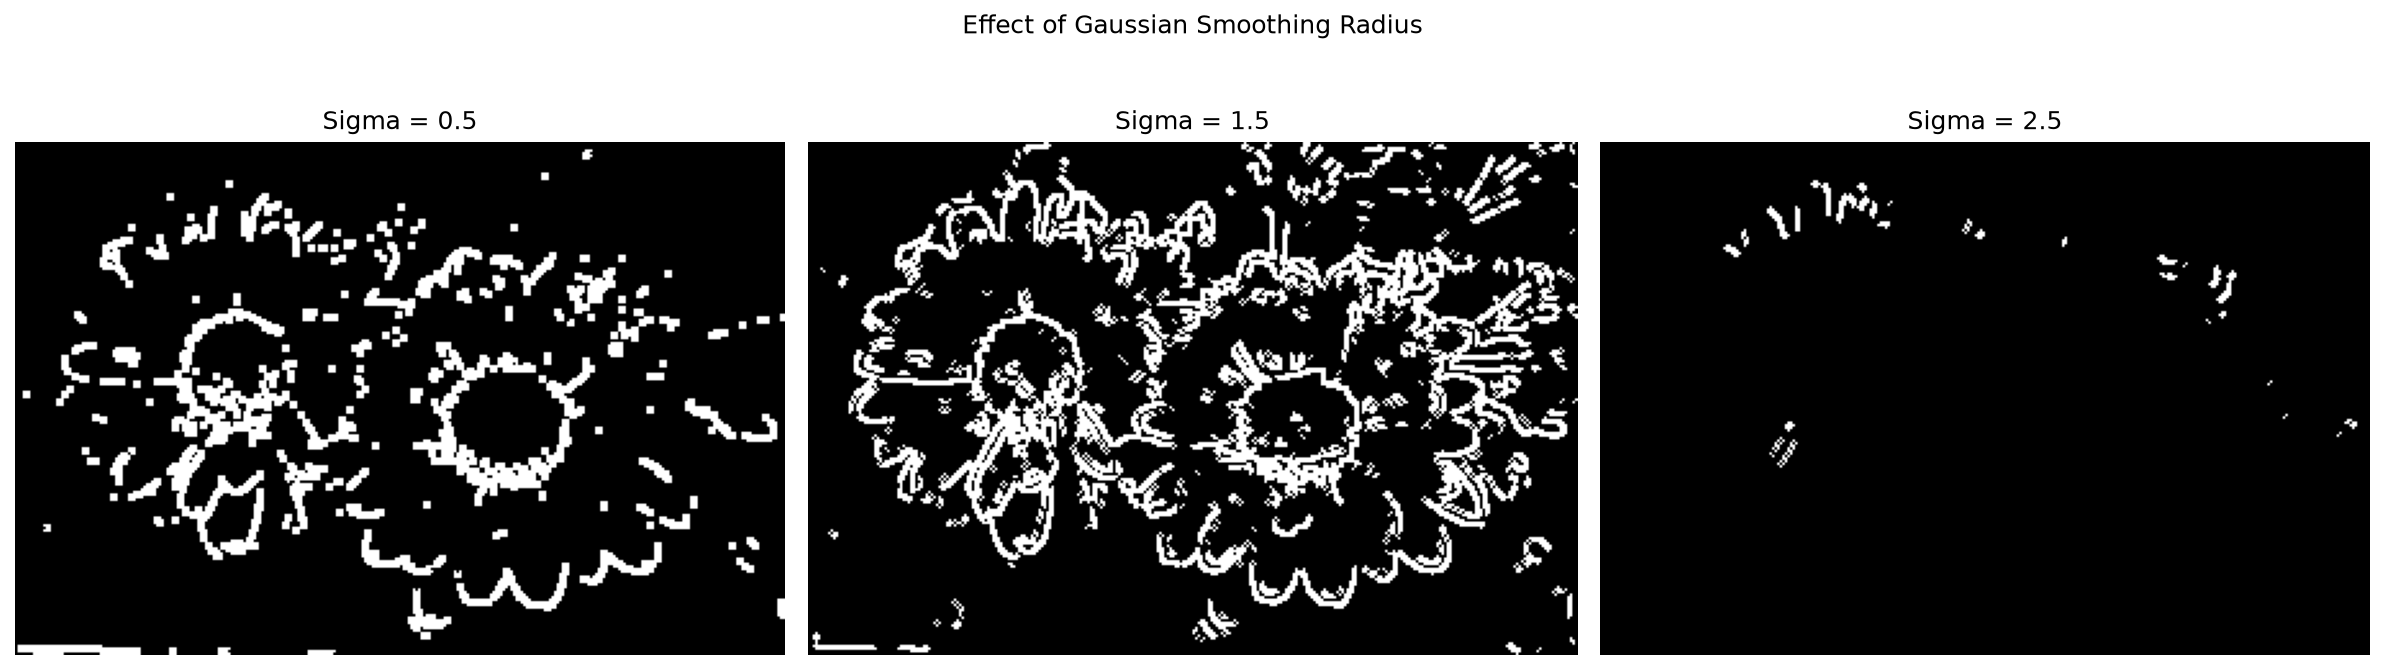
\includegraphics[width=\linewidth]{image1/gaussian_radius_effect.png}
    \caption{Effect of Gaussian smoothing radius $\sigma \in \{0.5, 1.5, 2.5\}$ with slope threshold held constant at $t = 0.015$. Increasing $\sigma$ transitions the detector from noisy micro-textures to coarse, delocalized macro-boundaries.}
    \label{fig:sigma_effect}
\end{figure}

\subsubsection{Effect of Slope Threshold ($t$)}

Figure below compares $t \in \{0.005,0.015,0.030\}$ at fixed $\sigma=1.5$:
\begin{itemize}
    \item \textbf{$t=0.005$:} Many weak crossings remain, creating dense responses in textured and shadowed regions.
    \item \textbf{$t=0.015$:} Most background noise is removed while major boundaries remain.
    \item \textbf{$t=0.030$:} Only stronger crossings remain, producing a sparser edge map.
\end{itemize}

\begin{figure}[H]
    \centering
    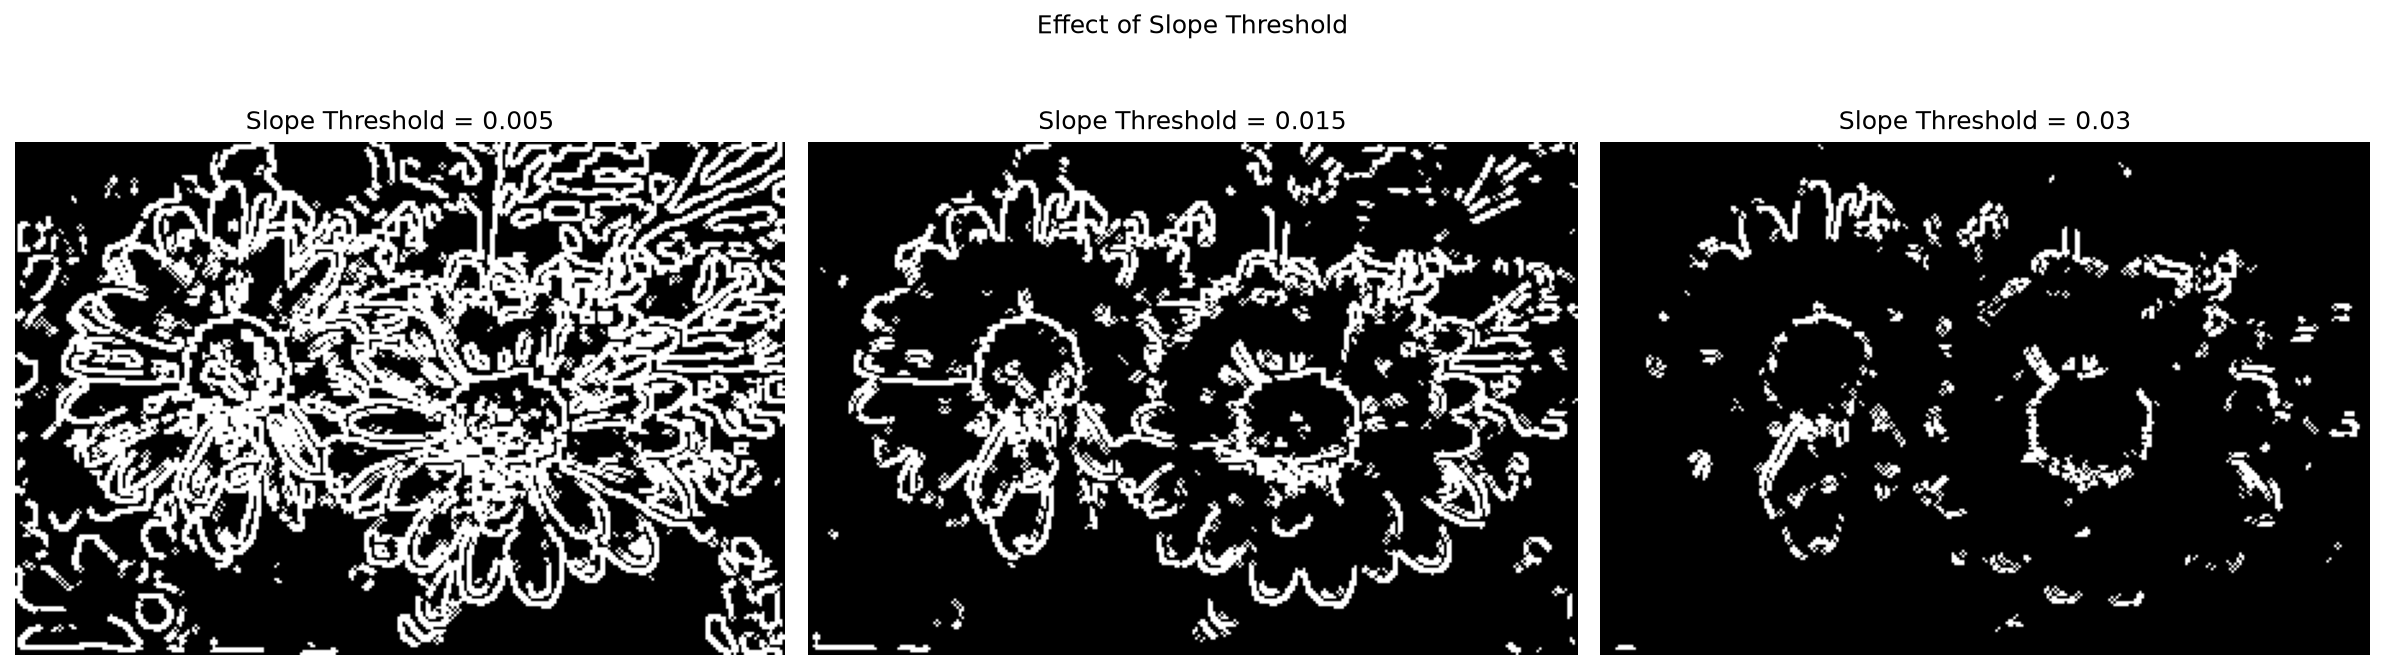
\includegraphics[width=\linewidth]{image1/slope_threshold_effect.png}
    \caption{Effect of slope threshold $t \in \{0.005, 0.015, 0.030\}$ with $\sigma = 1.5$. Raising $t$ filters out low-contrast background clutter while preserving salient foreground transitions.}
    \label{fig:threshold_effect}
\end{figure}


\section{Graph Construction and Feature-Based Cost Formulation}

We represent the image as a directed graph $G=(V,E)$. Each pixel $p=(y,x)$ is a vertex connected to its 8-connected neighbors $q$. The edge cost $c(p,q)$ is low near likely boundaries and high in less suitable regions.

\subsection{input image Feature Extraction}

We compute three feature maps:
\begin{enumerate}
    \item \textbf{Continuous Zero-Crossing Strength ($S_z$):} Rather than a binary thresholded mask, we assign each pixel a continuous strength based on the maximum LoG jump across adjacent sign flips:
    \[
    S_z(x,y) = \max_{(dx, dy) \in N_8} \Big\{ |\text{LoG}(x,y) - \text{LoG}(x+dx, y+dy)| \cdot \mathbb{I}\big(\text{LoG}(x,y) \cdot \text{LoG}(x+dx, y+dy) < 0\big) \Big\}
    \]
    We normalize the map to $[0,1]$ using its 99th percentile.
    \item \textbf{Gradient Magnitude ($G$):} Computed using Sobel kernels on a Gaussian-smoothed ($\sigma = 1.0$) luminance input image:
    \[
    G_x = \text{Sobel}_x(I_{\text{smooth}}), \quad G_y = \text{Sobel}_y(I_{\text{smooth}}), \quad G(x,y) = \sqrt{G_x^2 + G_y^2}
    \]
    We normalize it to $[0,1]$ using the 99th percentile.
    \item \textbf{Gradient Orientation ($\theta$):} The spatial direction of maximum intensity change:
    \[
    \theta(x,y) = \operatorname{atan2}(G_y(x,y), G_x(x,y))
    \]
\end{enumerate}

\begin{figure}[H]
    \centering
    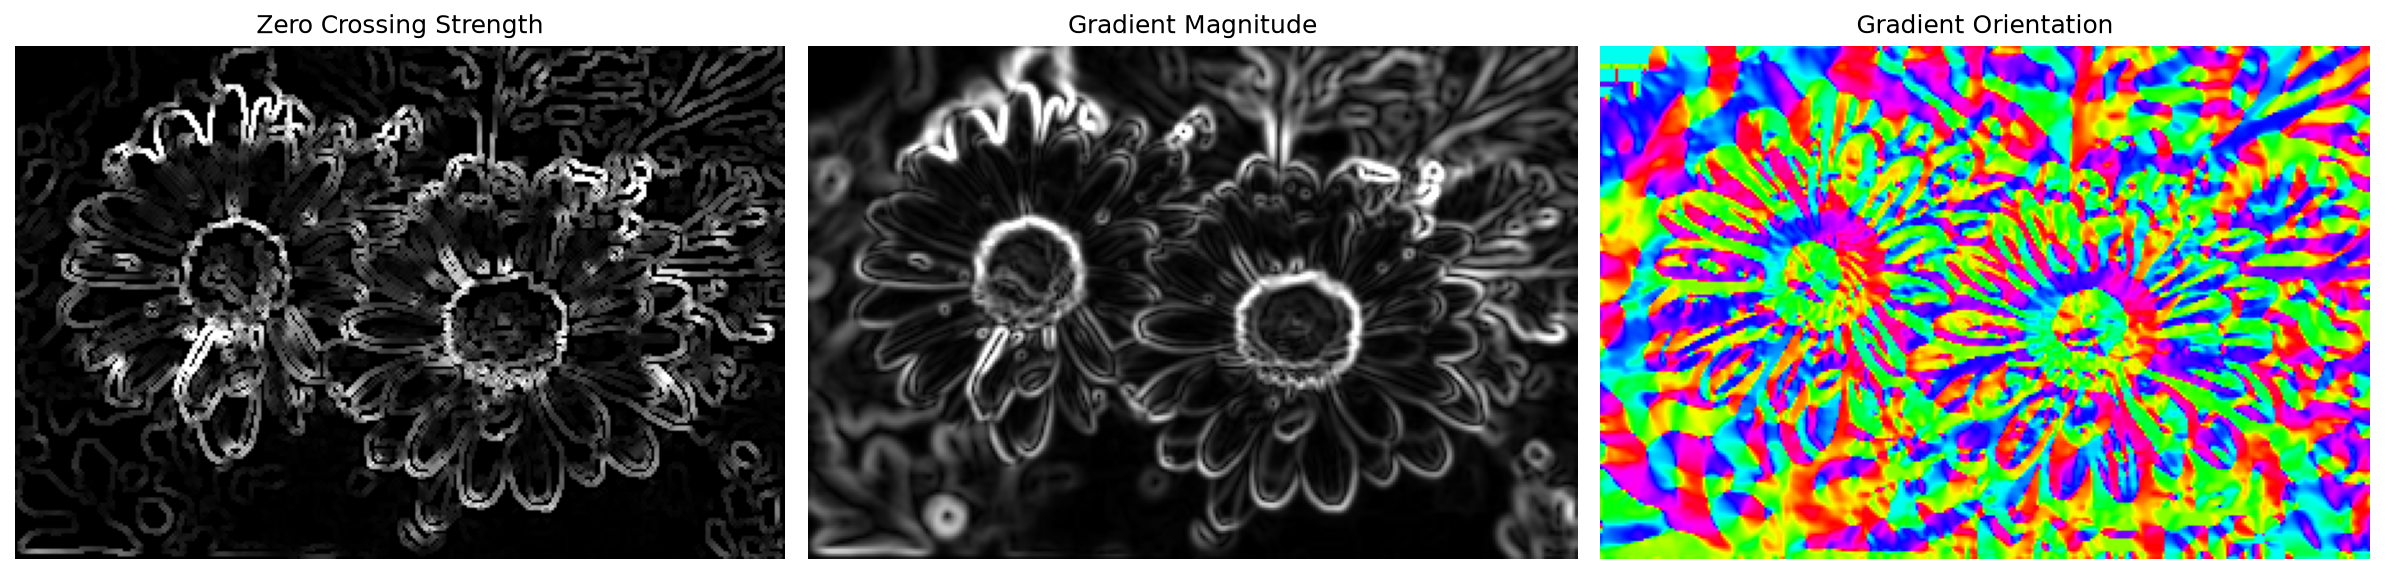
\includegraphics[width=\linewidth]{image1/gradient.png}
    \caption{Spatial feature maps used for edge cost formulation: (left) continuous LoG zero-crossing strength $S_z$, (center) gradient magnitude $G$, (right) gradient orientation $\theta$ displayed via cyclic HSV colormap.}
    \label{fig:gradient}
\end{figure}

\subsection{Local Edge Cost Terms}

For a link from $p=(y,x)$ to $q=(ny,nx)$, let $\mathbf d=(nx-x,ny-y)$ and $\hat{\mathbf d}=\mathbf d/\|\mathbf d\|_2$. The edge cost has three components:

\paragraph{1. Zero-Crossing Cost ($c_z$):} Inverse of the average zero-crossing strength at both link endpoints:
\[
c_z(p,q) = 1.0 - \frac{S_z(p) + S_z(q)}{2}
\]
Strong zero-crossings therefore have low cost.

\paragraph{2. Gradient Magnitude Cost ($c_g$):} High gradient magnitude indicates strong edge presence. Inverting this yields:
\[
c_g(p,q) = 1.0 - \frac{G(p) + G(q)}{2}
\]
Strong gradients therefore have low cost.

\paragraph{3. Gradient Direction Cost ($c_o$):} The image gradient $\nabla I=(G_x,G_y)$ is perpendicular to an edge, while movement along the boundary is tangential. Thus, the two directions should be orthogonal:
\[
\hat{\mathbf{g}} \cdot \hat{\mathbf{d}} = 0, \quad \text{where } \hat{\mathbf{g}} = \frac{\nabla I}{\|\nabla I\|_2}
\]
We measure this using the directional cost:
\[
c_o(p,q) = \frac{1}{2} \left( \left|\hat{\mathbf{g}}(p) \cdot \hat{\mathbf{d}}\right| + \left|\hat{\mathbf{g}}(q) \cdot \hat{\mathbf{d}}\right| \right)
\]
Movement along the edge gives zero cost, while movement across it gives maximum cost.

\paragraph{Combined Weighted Cost ($c_{\text{comb}}$):}
The combined cost is the weighted sum of the three terms, multiplied by the Euclidean step length to account for diagonal moves:
\[
c_{\text{comb}}(p,q) = \|\mathbf{d}\|_2 \cdot \left( w_z\,c_z(p,q) + w_g\,c_g(p,q) + w_o\,c_o(p,q) + \epsilon \right)
\]
We use $\epsilon=10^{-4}$ to keep edge costs positive. Unless stated otherwise, the weights are equal: $w_z=w_g=w_o=1/3$.


\section{Dijkstra's Algorithm and Cumulative Distance Analysis}

\subsection{Algorithmic Formulation}

We implement Dijkstra's algorithm using a min-heap, a distance array, a visited array, and a predecessor array for path reconstruction. With $V=HW$ vertices and at most $8V$ edges, its time complexity is $\mathcal{O}(E\log V)$. On our $200\times300$ image, a full search takes under 0.8 seconds.

\subsection{Distance Map Comparison Across Cost Regimes}

We run Dijkstra's algorithm from seed $s=(150,150)$ using four cost configurations:
\begin{enumerate}
    \item \textbf{Zero-crossing only:} Paths favor LoG zero-crossings but may leave the boundary where responses have gaps (Figure~\ref{fig:distance_map}a).
    \item \textbf{Gradient magnitude only:} Paths favor strong gradients but may drift across wide edge bands (Figure~\ref{fig:distance_map}b).
    \item \textbf{Orientation only:} Movement across the gradient direction is penalized (Figure~\ref{fig:distance_map}c).
    \item \textbf{Combined weights:} The three features provide complementary information and balance edge strength with direction (Figure~\ref{fig:distance_map}d).
\end{enumerate}

\begin{figure}[H]
    \centering
    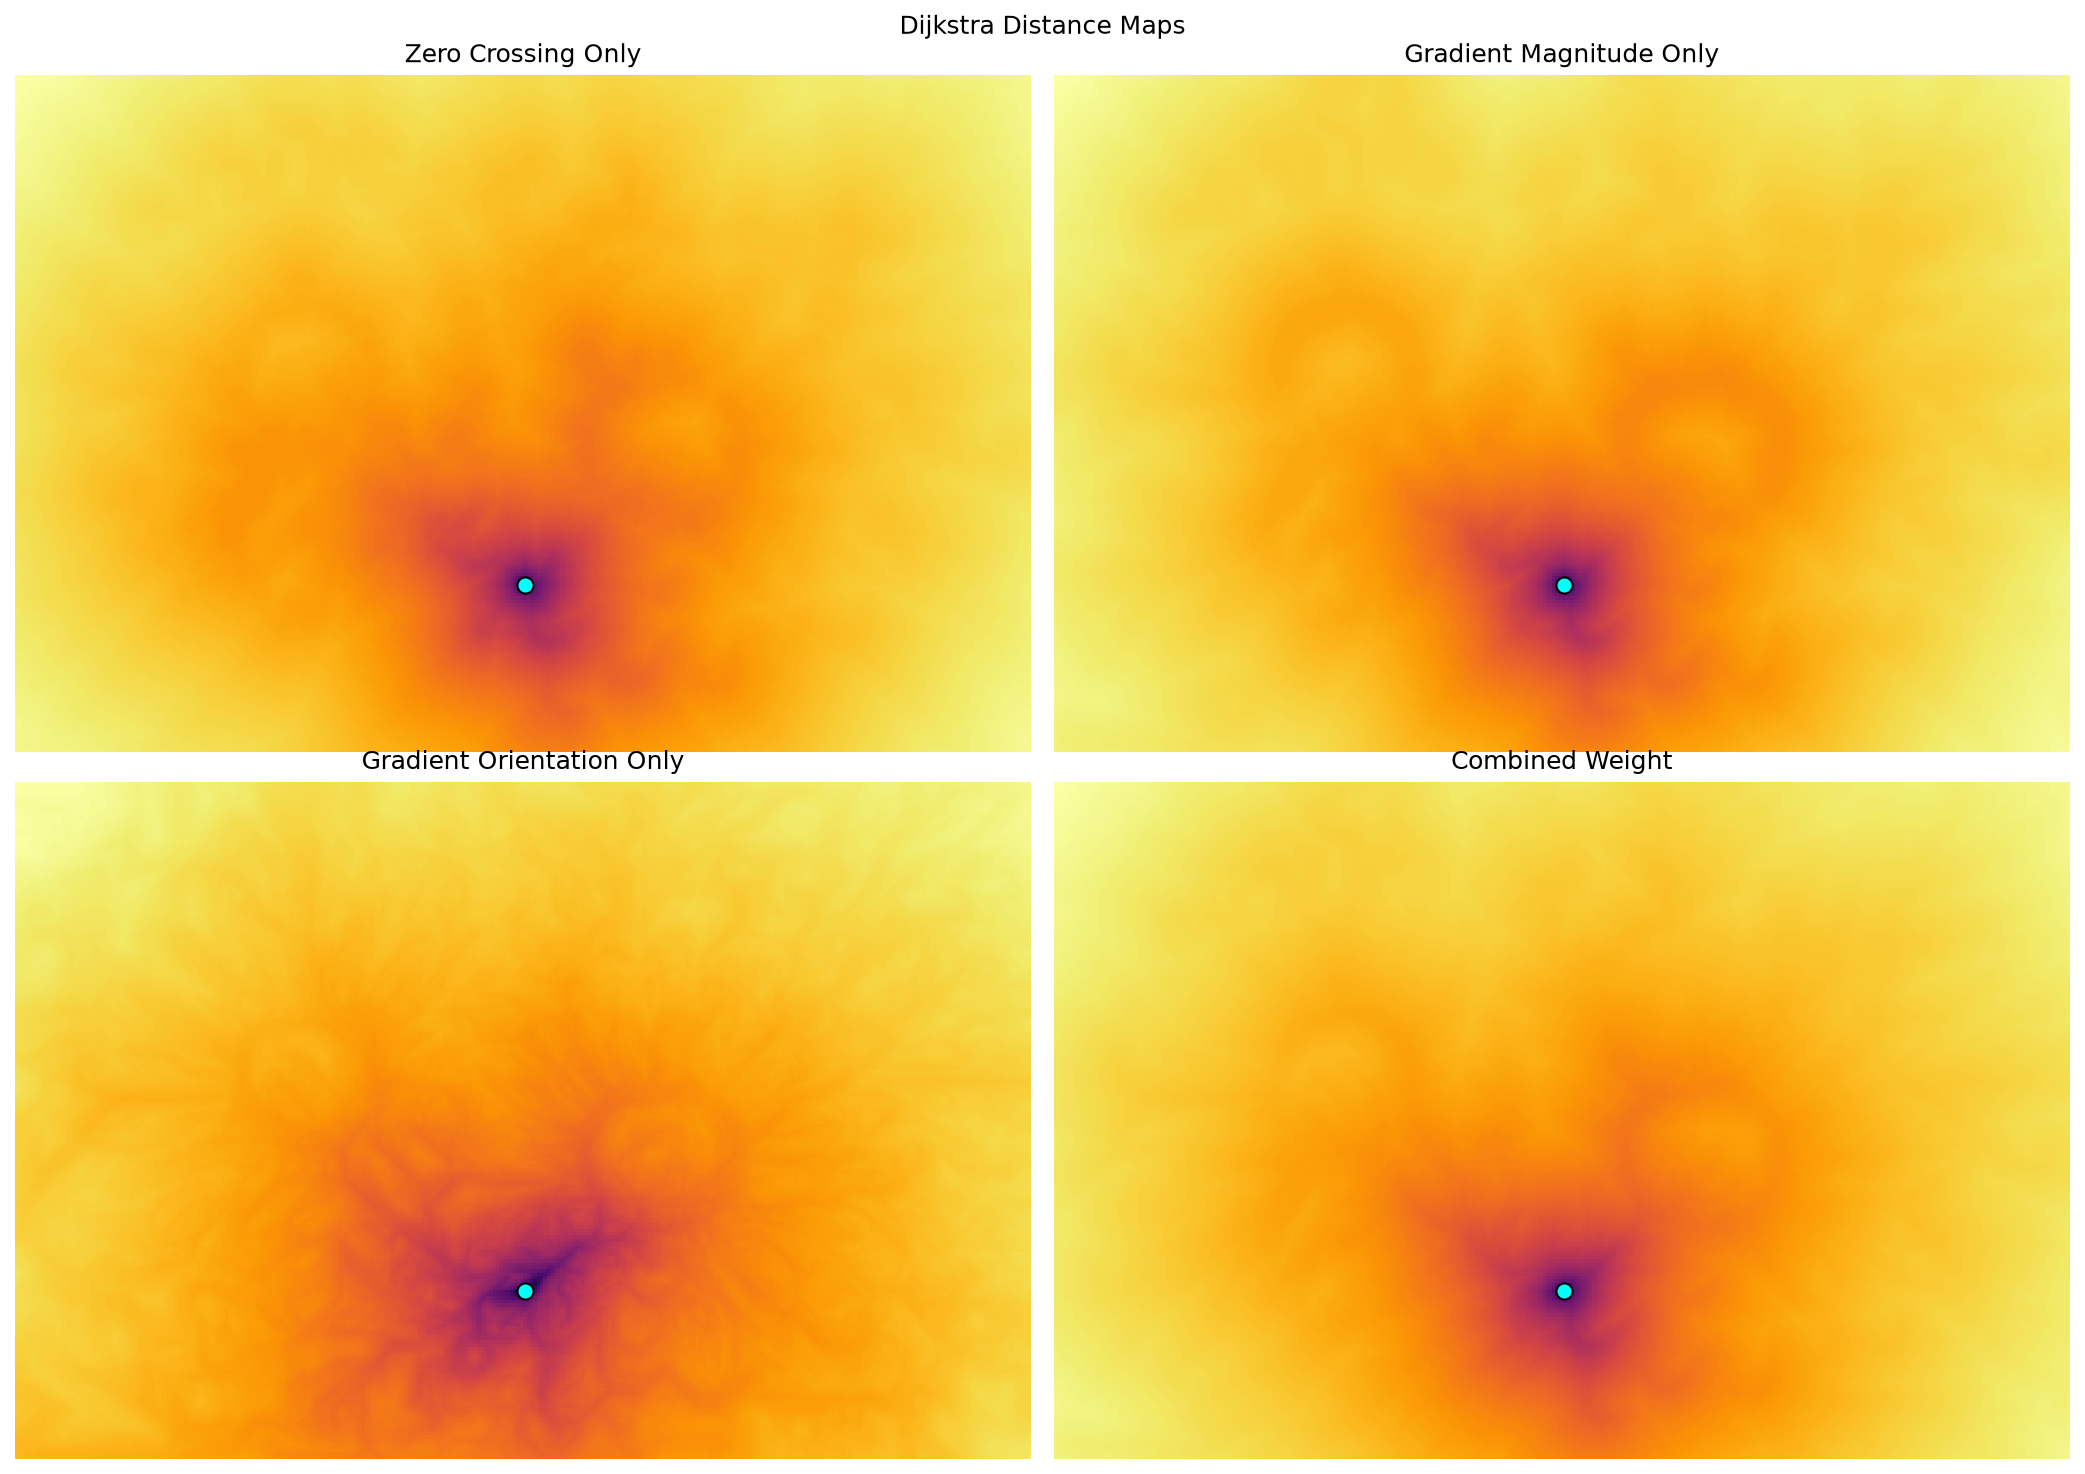
\includegraphics[width=0.72\linewidth]{image1/distance_map.png}
    \caption{Logarithmic cumulative distance maps $\log(1 + D)$ computed from seed $(150, 150)$ under four edge weight functions. Darker channels indicate low cumulative cost, revealing preferential wavefront propagation along object boundaries.}
    \label{fig:distance_map}
\end{figure}


\section{Interactive Segmentation Results}

\subsection{Seed Placement and Contour Snapping}

We manually place 16 seeds along the right flower's boundary. For each consecutive pair $S_i,S_{i+1}$, we run Dijkstra's algorithm until the target is reached and reconstruct the shortest path using predecessor pointers:
\[
p_k = P[p_{k+1}]
\]
Joining the paths produces a closed contour.

\begin{figure}[H]
    \centering
    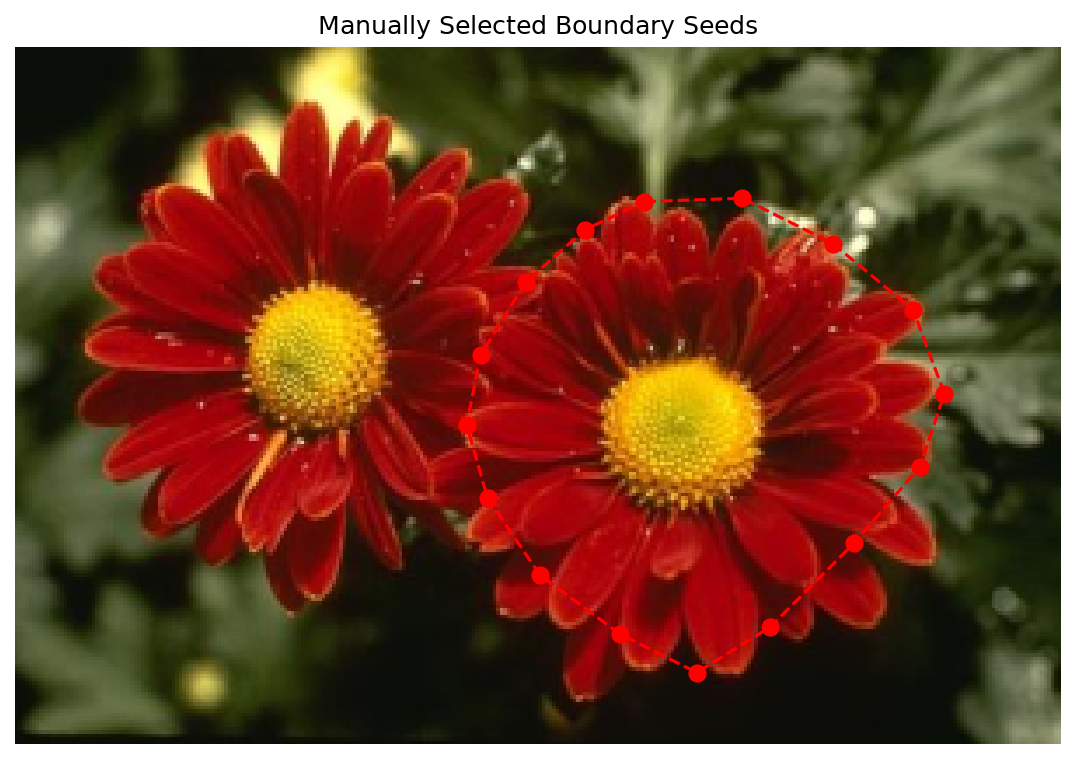
\includegraphics[width=0.5\linewidth]{image1/boundary_seed.png}
    \caption{Manually placed boundary seeds ($N=16$) overlaid on the input image with dashed linear segments connecting consecutive seed pairs prior to shortest-path optimization.}
    \label{fig:boundary_seed}
\end{figure}

\subsection{Segmentation Mask Generation}

We rasterize the closed contour $\mathcal C=\{(y_k,x_k)\}_{k=1}^K$ into a binary mask $M$ using OpenCV's polygon-filling function. The foreground is then extracted by pixel-wise masking:
\[
I_{\text{seg}}(y,x) = M(y,x) \cdot I(y,x)
\]
Figure below shows the selected seeds, shortest-path contour, and extracted flower.

\begin{figure}[H]
    \centering
    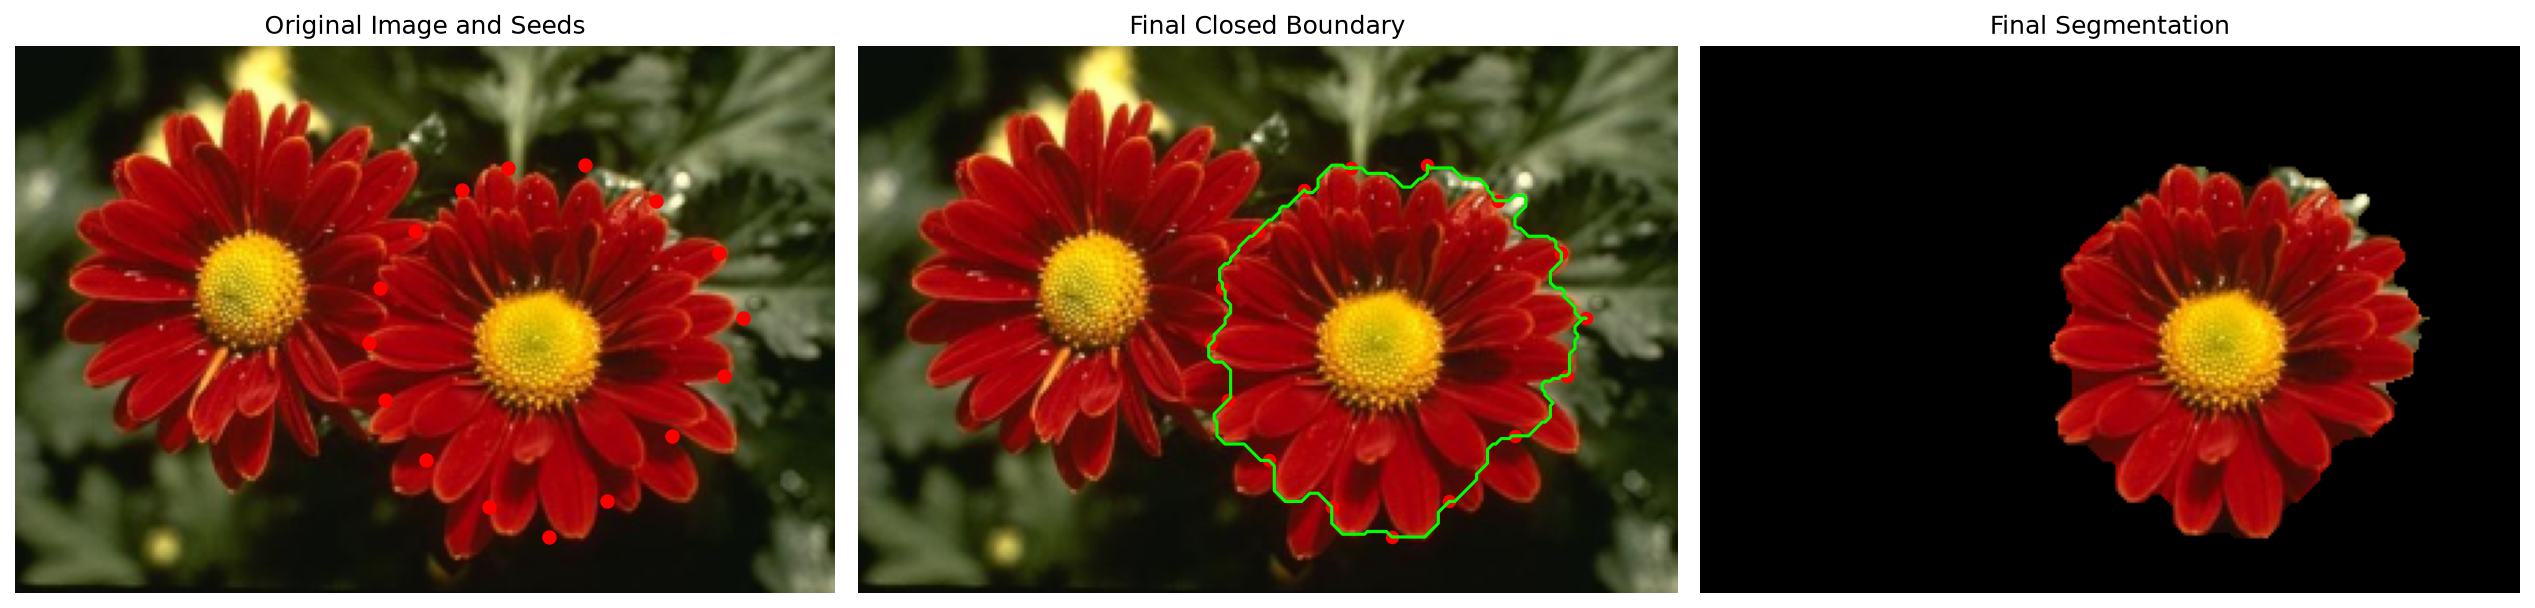
\includegraphics[width=\linewidth]{image1/segmentation_marr.png}
    \caption{Interactive segmentation results using Marr-Hildreth Intelligent Scissors: (left) seeds, (center) live-wire optimal contour snapping to petal edges, (right) final extracted foreground flower.}
    \label{fig:segmentation_marr}
\end{figure}


\section{Edge Weight Modifications and Evaluation}

We evaluate two modifications to the edge cost function.

\subsection{Modification 1: Canny Edge Detector Integration}

We replace the LoG zero-crossing feature $S_z$ with a binary map from the \textbf{Canny edge detector}, using thresholds $T_{\text{low}}=50$ and $T_{\text{high}}=150$. Canny applies:
\begin{enumerate}
    \item Non-maximum suppression (NMS) along the gradient direction to enforce 1-pixel thin edge ridges.
    \item Hysteresis thresholding with two limits to eliminate spurious isolated edges while maintaining edge continuity.
\end{enumerate}

Figure below compares the two edge features, and Figure~\ref{fig:segmentation_canny} shows the resulting segmentation.

\begin{figure}[H]
    \centering
    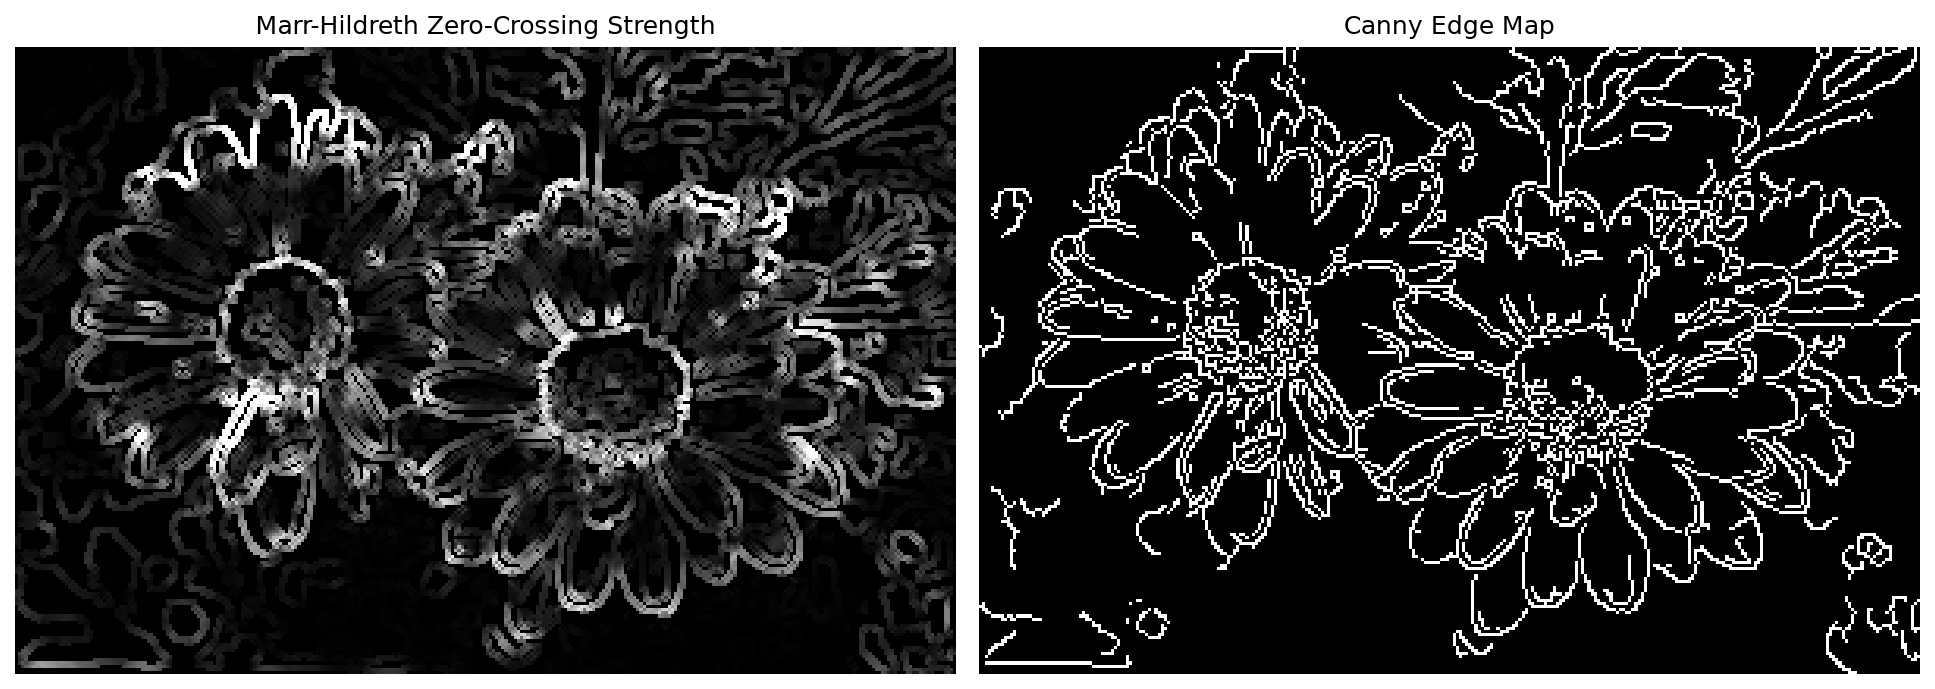
\includegraphics[width=0.75\linewidth]{image1/canny_vs_marr.png}
    \caption{Comparison of edge feature representations: (left) continuous LoG zero-crossing strength map, (right) Canny edge map after non-maximum suppression and hysteresis.}
    \label{fig:canny_comp}
\end{figure}

\begin{figure}[H]
    \centering
    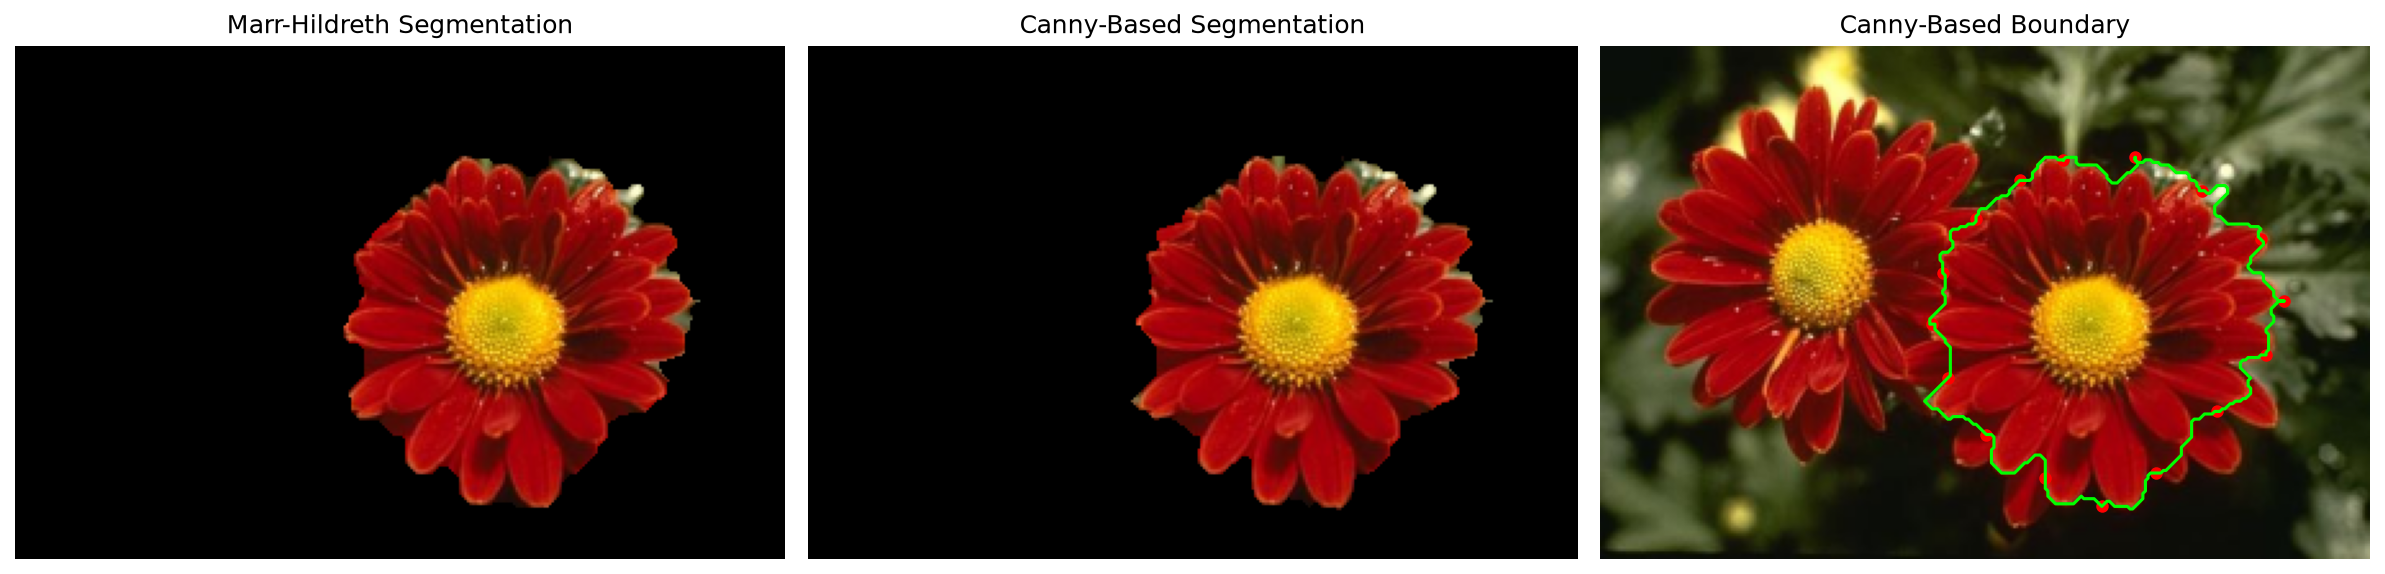
\includegraphics[width=\linewidth]{image1/segmentation_canny.png}
    \caption{Segmentation comparison: (left) Marr-Hildreth baseline, (center) Canny-based segmentation, (right) Canny-based live-wire boundary.}
    \label{fig:segmentation_canny}
\end{figure}

\subsection{Modification 2: Weight Vector Rebalancing}

The baseline uses equal weights, $\mathbf{w}_{\text{orig}}=(1/3,1/3,1/3)$. We compare these with weights that emphasize zero-crossings:
\[
\mathbf{w}_{\text{mod}} = (w_z, w_g, w_o) = (0.8, 0.1, 0.1)
\]
Figure below compares the resulting boundaries:
\begin{itemize}
    \item \textbf{Equal weights:} Gradient magnitude and orientation help guide paths where zero-crossings are weak.
    \item \textbf{Zero-crossing emphasized:} The path relies more strongly on zero-crossings and may become less smooth in textured regions.
\end{itemize}

\begin{figure}[H]
    \centering
    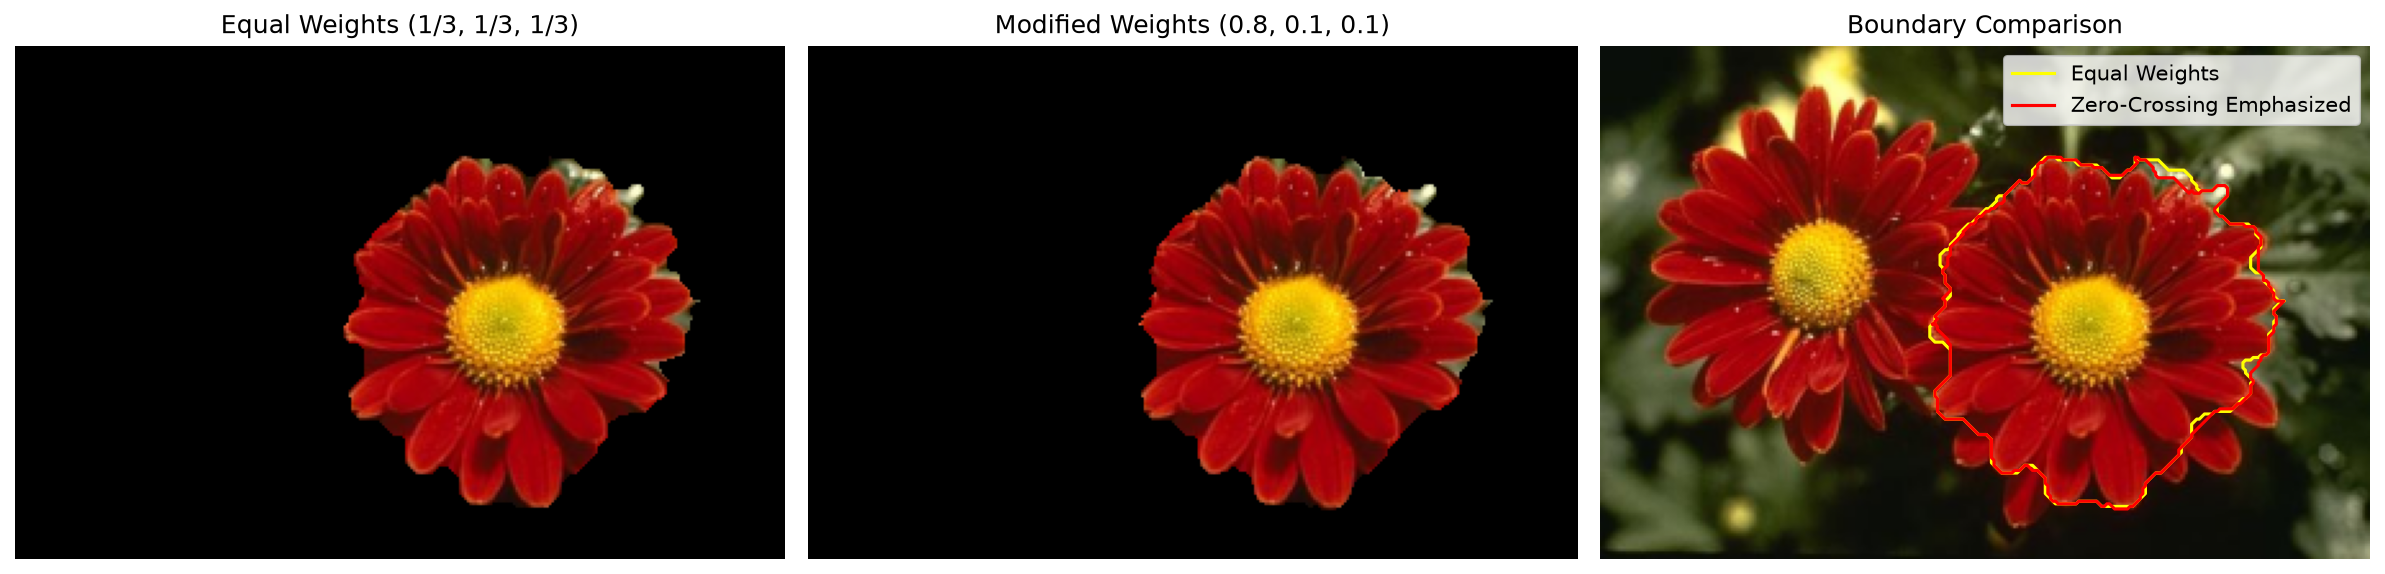
\includegraphics[width=\linewidth]{image1/og_vs_modified_weight.png}
    \caption{Impact of weight parameter rebalancing: (left) baseline equal weights ($1/3, 1/3, 1/3$), (center) zero-crossing prioritized ($0.8, 0.1, 0.1$), (right) side-by-side boundary overlay (yellow = equal weights, red = zero-crossing emphasized).}
    \label{fig:weight_comp}
\end{figure}


\section{Discussion, Computational Complexity, and Limitations}

\subsection{Algorithmic Complexity and Scalability}

The main computational costs arise from edge detection, feature extraction, and shortest-path searches:
\begin{table}[H]
\centering
\small
\setlength{\tabcolsep}{4pt}
\renewcommand{\arraystretch}{1.3}

\begin{tabularx}{\textwidth}{
    >{\raggedright\arraybackslash}p{0.19\textwidth}
    >{\centering\arraybackslash}p{0.24\textwidth}
    >{\centering\arraybackslash}p{0.29\textwidth}
    >{\centering\arraybackslash}X
}
\toprule
\textbf{Pipeline Stage} &
\textbf{Algorithm / Method} &
\textbf{Theoretical Complexity} &
\textbf{Empirical Runtime} \\
\midrule

LoG Edge Detection
& 2D Separable Gaussian Filtering
& $\mathcal{O}(H \cdot W \cdot K_\sigma)$
& $= 12$ ms \\

Gradient and Feature Extraction
& Sobel Kernels + Vector Math
& $\mathcal{O}(H \cdot W)$
& $= 8$ ms \\

Single Dijkstra Propagation
& Min-Heap Priority Queue
& $\mathcal{O}(V \log V + E)$
& $= 180$ ms \\

Interactive Segment (Targeted)
& Early-Exit Dijkstra
& $\mathcal{O}(V_{\text{explored}} \log V_{\text{explored}})$
& $= 35$ ms / seed \\

Total Contour Extraction
& 16 Interactive Seed Connections
& $\sum_{i=1}^{16} \mathcal{O}(E_i \log V_i)$
& $= 0.52$ s \\

\bottomrule
\end{tabularx}

\caption{Computational complexity and empirical runtime across each pipeline stage.}
\label{tab:runtime}
\end{table}

Stopping Dijkstra's search when the destination is reached avoids exploring the entire image for each seed pair.

\subsection{Failure Modes and Limitations}

The method has several limitations:
\begin{enumerate}
    \item \textbf{Sparse seeds:} Seeds placed too far apart may allow the shortest path to cut across deep concavities.
    \item \textbf{Low contrast:} Weak object boundaries can cause paths to follow stronger nearby background edges.
    \item \textbf{LoG delocalization:} Large smoothing radii can shift zero-crossings away from the actual boundary.
\end{enumerate}




\end{document}